\documentclass[12pt,a4paper]{report}

%--------------------------------------
\usepackage[T1]{fontenc} %Not needed by LuaLaTeX or XeLaTeX
%--------------------------------------

%Portuguese-specific commands
%--------------------------------------
%\usepackage[portuguese]{babel}
%--------------------------------------

%Hyphenation rules
%--------------------------------------
\usepackage{hyphenat}
\hyphenation{mate-mática recu-perar}
%--------------------------------------

%Espaçamento e outras cenas
%--------------------------------------
\usepackage{setspace}
\usepackage{anyfontsize}
\usepackage{indentfirst}
\usepackage{parskip}
\usepackage{titlesec} % Chapter
\usepackage{geometry} % Margens
\usepackage{amsmath} % Matemática
\usepackage{graphicx}
\usepackage{wrapfig}
\usepackage{subcaption}
\usepackage{caption}
\usepackage[hidelinks]{hyperref}
\usepackage{xpatch}
\usepackage{etoolbox}
\usepackage{titletoc}
\usepackage{times}
\usepackage{fancyhdr}
\usepackage{lastpage}
\usepackage{xcolor}
\usepackage{listings}
\usepackage{tabularx}
\usepackage{array}
%------------------------------

%Margens
\geometry{
    a4paper,
    right = 3cm,
    left = 2.5cm,
    top = 2.5cm,
    bottom = 2.5cm,
}

\renewcommand{\contentsname}{Índice}
\newcommand{\code}{\texttt\textbf}

\setcounter{secnumdepth}{0} % Não enumerar secções

\setstretch{1.5} % espaçamento

\titleformat{\chapter}{\fontfamily{ptm}\selectfont\centering\huge\titlerule[1.5pt]\vspace{-9pt}}{}{0pt}{\Huge}[{\titlerule[1.5pt]}]

\titleformat{\section}{\bfseries\fontfamily{ptm}\selectfont}{}{0pt}{\large}[{\titlerule[1pt]}]

\titleformat{\subsection}{\bfseries\fontfamily{ptm}\selectfont}{}{0pt}{\large}[\vspace{2pt}]


\titlespacing{\chapter}{0pt}{-30pt}{30pt}


\titlecontents{section}[40pt]{\vskip3pt\bfseries}{\thecontentslabel\quad}{}{~~\normalfont\dotfill\bfseries\contentspage}[]

\newcolumntype{P}[1]{>{\centering\arraybackslash}p{#1}}

\begin{document}


\chapter{Introdução}

Quando estamos perante uma situação na qual temos de lidar com a manipulação de grandes quantidades de dados existem sempre algumas opções que devemos preferir adotar e outras que, pelo contrário, devemos evitar a todo o custo, portanto, ao longo deste relatório iremos explicar as estratégias que utilizámos para abordar este problema, e porque razão optámos por uma estratégia em específico e não outra qualquer.

Posto isto, importa também realçar que nas estruturas que iremos exemplificar mais à frente tivemos em conta a natureza dos dados com os quais estávamos a lidar e as questões que tinham de ser resolvidas em tempo útil, assim sendo, caso levássemos em conta outros quaisquer fatores, certamente a abordagem adotada teria sido diferente.

\chapter{Catálogos}

Antes de mais, a primeira etapa do projeto diz respeito ao armazenamento dos dados, ou seja, tínhamos de guardar toda a informação útil numa determinada estrutura, portanto, como reparámos que existem três entidades fundamentais \textit{(users, drivers, rides)}, decidimos criar uma estrutura de dados para cada uma destas entidades, e mais uma para as cidades, visto que em várias \textit{queries} as cidades são um dos parâmetros visados.

\section{Utilizadores}

\begin{figure}[h]
    \centering
    \begin{subfigure}{\textwidth}
        \centering
        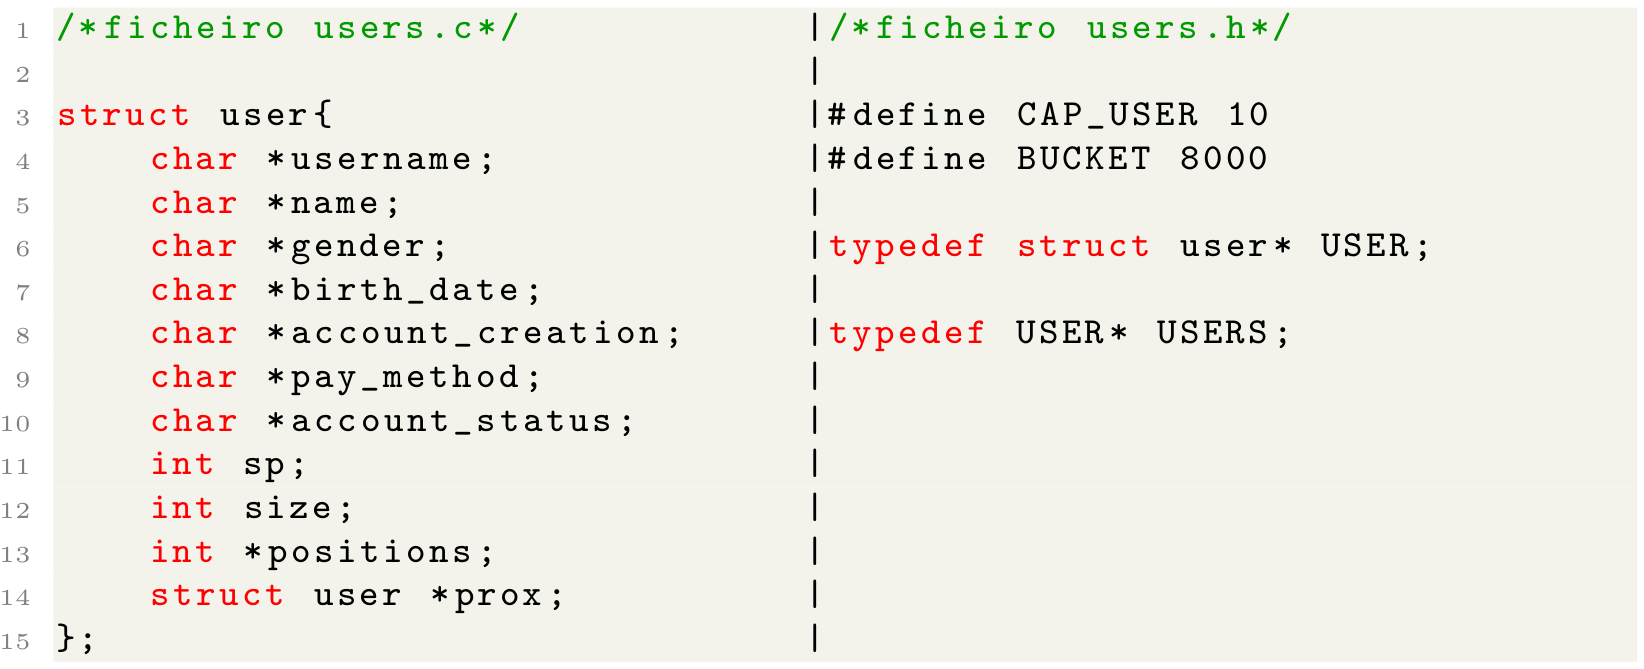
\includegraphics[width=1\linewidth]{images/users.png}
        \caption*{Estrutura de dados dos utilizadores}
        \label{fig:users}
    \end{subfigure}
\end{figure}

Tal como é possível observar pela estrutura presente no ficheiro \textit{users.c}, um utilizador é um elemento de uma lista ligada, visto que um dos campos corresponde a um apontador para outro \texttt{\small\textbf{struct user}}. Além disso, existe mais um campo em particular para além daqueles que, como estão presentes no ficheiro \textit{users.csv}, teriam de estar aqui obrigatoriamente, falamos nem mais nem menos do campo \texttt{\small\textbf{positions}}. Este corresponde a um \textit{array} dinâmico que começa com um tamanho definido por \textbf{\small\texttt{CAP\_USER}}, e conforme o valor do \textbf{\small\texttt{sp}} (número de elementos do \textit{array}) iguala o do \textbf{\small\texttt{size}}, este último multiplica por dois, sendo que os elementos do \textit{array} equivalem a todas as posições em que um determinado utilizador aparece no \textit{array} das viagens.

Passando para o ficheiro \textit{users.h}, percebe-se de que forma os utilizadores estão organizados, neste caso, os utilizadores são guardados numa tabela de \textit{hash}, onde cada utilizador é mapeado para uma determinada posição conforme o seu \texttt{\small\textbf{username}}, e acrescentado no início de uma lista ligada para poupar o máximo de tempo possível. Assim, a estrutura \texttt{\small\textbf{USERS}} corresponde a uma tabela de \textit{hash} com 8000 \textit{buckets}, onde cada utilizador pode ser acedido em tempo praticamente constante, não sendo constante pois é necessário percorrer um \textit{bucket}.


\normalsize\textbf{Vantagens}
    \begin{enumerate}
        \item Ao utilizar uma tabela de \textit{hash} podemos encontrar um utilizador mais facilmente, uma vez que a função de \textit{hash} mapeia apenas para um determinado \textit{bucket}.

        \item Com a utilização de uma lista ligada em cada um dos \textit{buckets} é possível inserir um utilizador no início da lista em tempo constante, algo que não seria possível num \textit{array}.
        
        \item Ao usufruir de uma lista ligada apenas vamos alocar a quantidade exata de memória necessária para representar os nossos dados em cada um dos \textit{buckets}. 
    \end{enumerate}

\normalsize\textbf{Desvantagens}
    \begin{enumerate}
        \item A utilização de listas ligadas não tira partido da localidade espacial, dado que os apontadores para os próximos elementos da lista estão dispersos na memória, como tal, a \textit{miss rate} aumenta, e portanto demoramos mais tempo a aceder ao elemento seguinte.
        
        \item Para libertar toda a memória que uma tabela de \textit{hash} ocupa é necessário despender algum tempo, visto que temos que percorrer as listas ligadas presentes em cada um dos \textit{buckets}.
    \end{enumerate}

\vspace{-0.35cm}
\section{Condutores}

\begin{figure}[hbt!]
    \centering
    \begin{subfigure}{\textwidth}
        \centering
        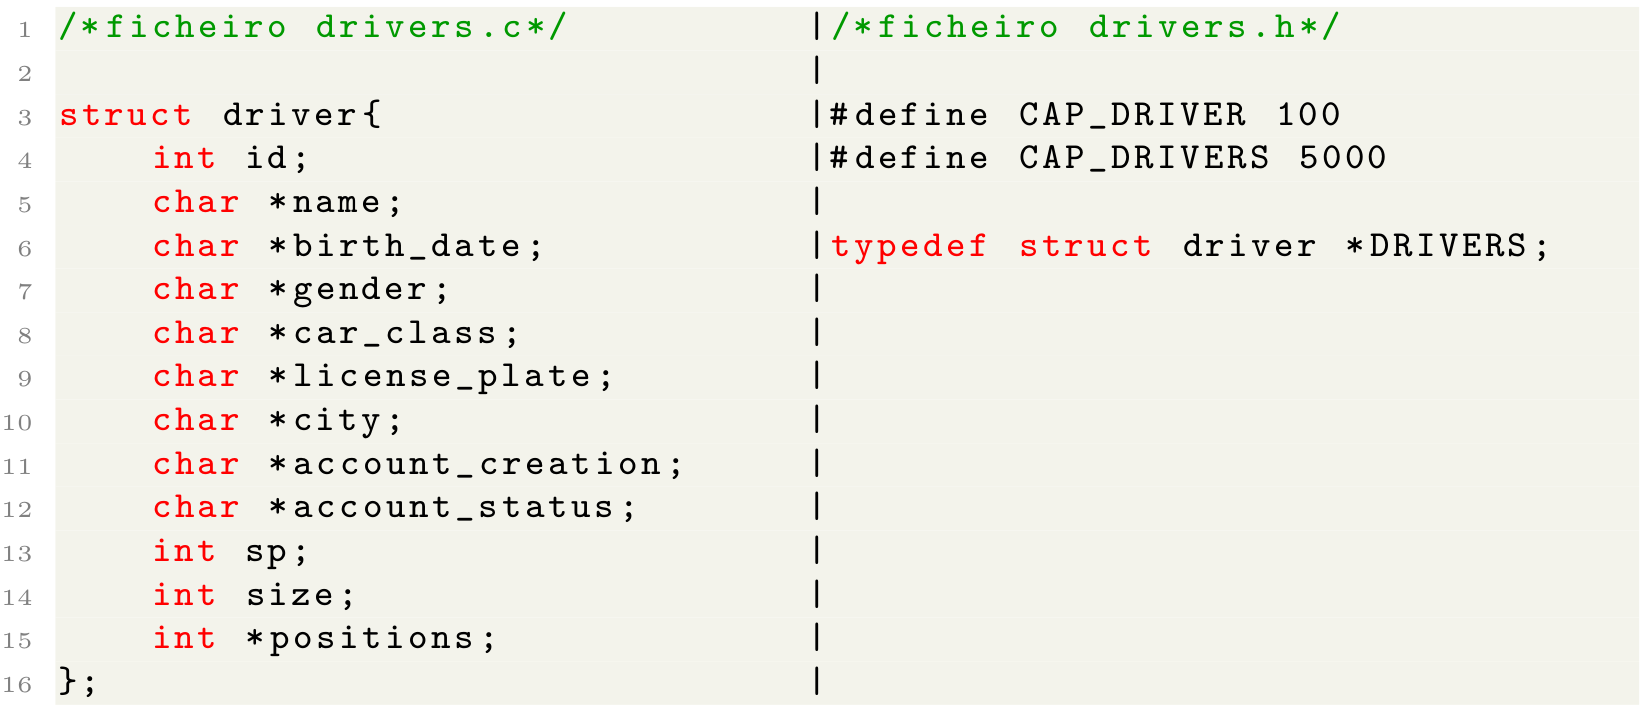
\includegraphics[width=1\linewidth]{images/drivers.png}
        \caption*{Estrutura de dados dos condutores}
        \label{fig:drivers}
    \end{subfigure}
\end{figure}

Agora na estrutura dos condutores, a estratégia adotada foi muito parecida à dos utilizadores, mais uma vez, todos os campos que estão presentes no ficheiro \textit{drivers.csv} também estão aqui presentes, e, além disso, também existe outro \textit{array} dinâmico \textbf{\small\texttt{positions}}, que a exemplo do anterior possui um tamanho inicial definido por \textbf{\small\texttt{CAP\_DRIVER}}, e tem como elementos todas as posições em que um determinado condutor aparece no \textit{array} das viagens.

De seguida, passando ao ficheiro \textit{drivers.h}, vemos que a estrutura \textbf{\small\texttt{DRIVERS}} é um \textit{array} dinâmico de tamanho inicial definido por \textbf{\small\texttt{CAP\_DRIVERS}}, onde cada elemento é um condutor. Neste caso, a forma de mapeamento utilizada para colocar um determinado condutor numa posição do \textit{array} foi o \textbf{\small\texttt{id}} do mesmo, ou seja, um condutor com um \textbf{\small\texttt{id}} correspondente a \textbf{\small\texttt{000000000162}}, será mapeado na posição de índice \textbf{\small\texttt{162}} do \textit{array} \textbf{\small\texttt{DRIVERS}}.


\normalsize\textbf{Vantagens}
    \begin{enumerate}
        \item A utilização de um \textit{array} tira partido da localidade espacial, o que aumenta o \textit{hit rate}, e consequentemente leva a um ganho de tempo, caso pretendamos percorrer o \textit{array}.
        
        \item Com um \textit{array} dinâmico nunca corremos o risco de alocar uma quantidade de memória muito maior do que aquela que é extremamente necessária, no pior dos casos alocamos o dobro daquela que seria pretendida.
        
        \item Quando pretendermos libertar a memória do \textit{array} \textbf{\small\texttt{DRIVERS}} não vai ser necessário percorrer o \textit{array}, ao contrário da tabela de \textit{hash}, neste caso a operação de libertar memória será feita em tempo constante.
        
        \item Se pretendermos aceder a um determinado utilizador, é possível fazer essa operação em tempo constante desde que saibamos, previamente, qual o \textbf{\small\texttt{id}} do condutor em questão.
    \end{enumerate}

\normalsize\textbf{Desvantagens}
    \begin{enumerate}
        \item A menos que saibamos qual o índice de um determinado condutor, teremos de percorrer o \textit{array} \textbf{\small\texttt{DRIVERS}} até encontrar o condutor que pretendemos.

        \item Ao usufruir desta forma de mapeamento, a posição de índice zero estará sempre vazia, uma vez que nenhum condutor tem um \textbf{\small\texttt{id}} equivalente a zero.
    \end{enumerate}

\pagebreak
\section{Viagens}

\begin{figure}[hbt!]
    \centering
    \begin{subfigure}{\textwidth}
        \centering
        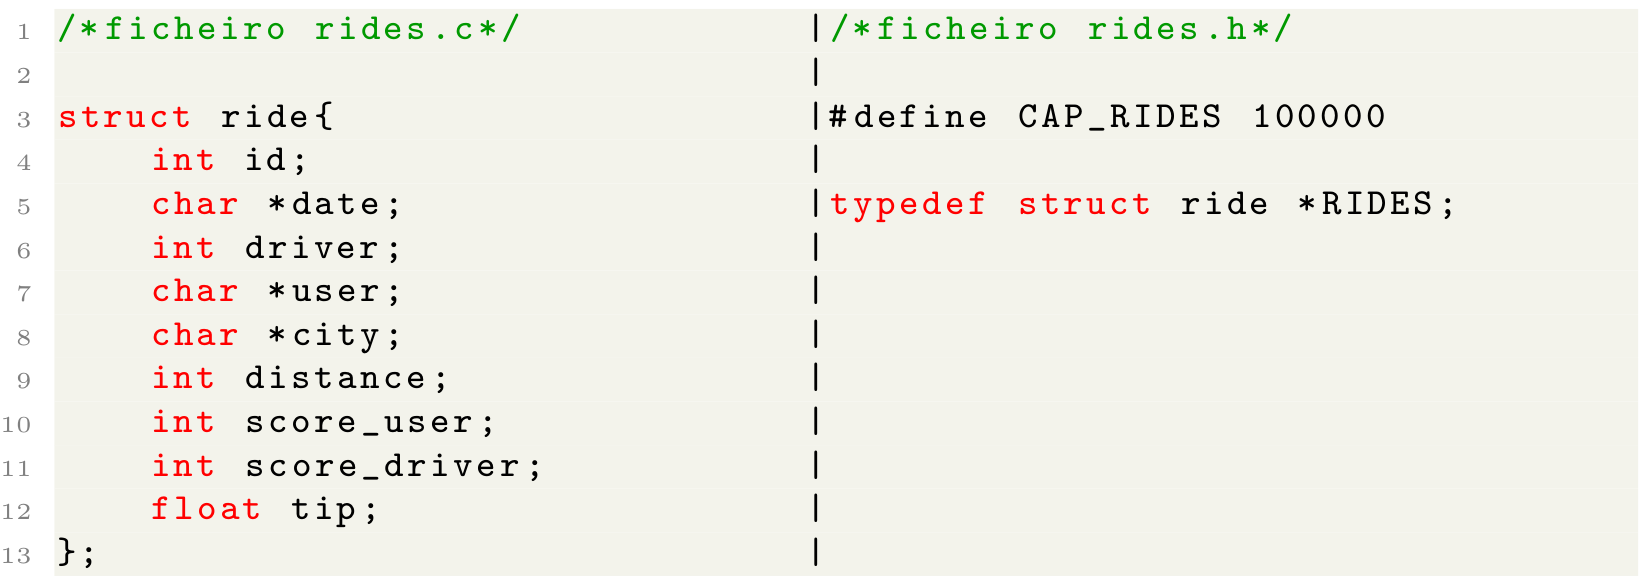
\includegraphics[width=1\linewidth]{images/rides.png}
        \caption*{Estrutura de dados das viagens}
        \label{fig:rides}
    \end{subfigure}
\end{figure}

Passando agora à estrutura das viagens, vemos que uma viagem possui apenas os campos presentes no ficheiro \textit{rides.csv}, e ao contrário das estruturas anteriores, não possui nenhum \textit{array} de inteiros.

Assim, a estrutura \textbf{\small\texttt{RIDES}} está implementada como sendo um \textit{array} dinâmico com tamanho inicial definido por \textbf{\small\texttt{CAP\_RIDES}}, onde cada elemento é uma viagem. E, novamente, a forma de mapeamento utilizada para determinar qual a posição de uma viagem, é o \textbf{\small\texttt{id}} da mesma, ou seja, uma viagem com um \textbf{\small\texttt{id}} correspondente a \textbf{\small\texttt{000000008439}} é inserida na posição de índice \textbf{\small\texttt{8439}} do \textit{array} \textbf{\small\texttt{RIDES}}.

\normalsize\textbf{Vantagens}
\begin{itemize}
   
    \item Quando for pretendido percorrer o \textit{array} \textbf{\small\texttt{RIDES}}, o programa vai beneficiar da localidade espacial, ou seja, será necessário menos tempo para percorrer as suas posições, dado que os endereços estarão em \textit{cache}.
    
    \item Se pretendermos aceder a uma determinada viagem, essa operação pode ser feita em tempo constante, caso saibamos previamente qual o \textbf{\small\texttt{id}} da viagem em questão, uma vez que as viagem são mapeadas conforme o seu \textbf{\small\texttt{id}}.

    \item Para libertar a memória alocada pelo \textit{array} \textbf{\small\texttt{RIDES}} não é necessário percorrer o mesmo.

    \item Como o \textit{array} \textbf{\small\texttt{RIDES}} é dinâmico, no pior dos casos é alocada o dobro da memória considerada necessária.
\end{itemize}

\pagebreak
\normalsize\textbf{Desvantagens}
\begin{itemize}
    \item Sem saber qual o \textbf{\small\texttt{id}} de uma viagem é necessário percorrer o \textit{array} \textbf{\small\texttt{RIDES}} para encontrar aquilo que pretendemos.
    
    \item A exemplo do que acontece no \textit{array} \textbf{\small\texttt{DRIVERS}}, também o \textit{array} \textbf{\small\texttt{RIDES}} possui a primeira posição vazia, ou seja, no índice zero não existe qualquer elemento.
\end{itemize}


\section{Cidades}

\begin{figure}[hbt!]
    \centering
    \begin{subfigure}{\textwidth}
        \centering
        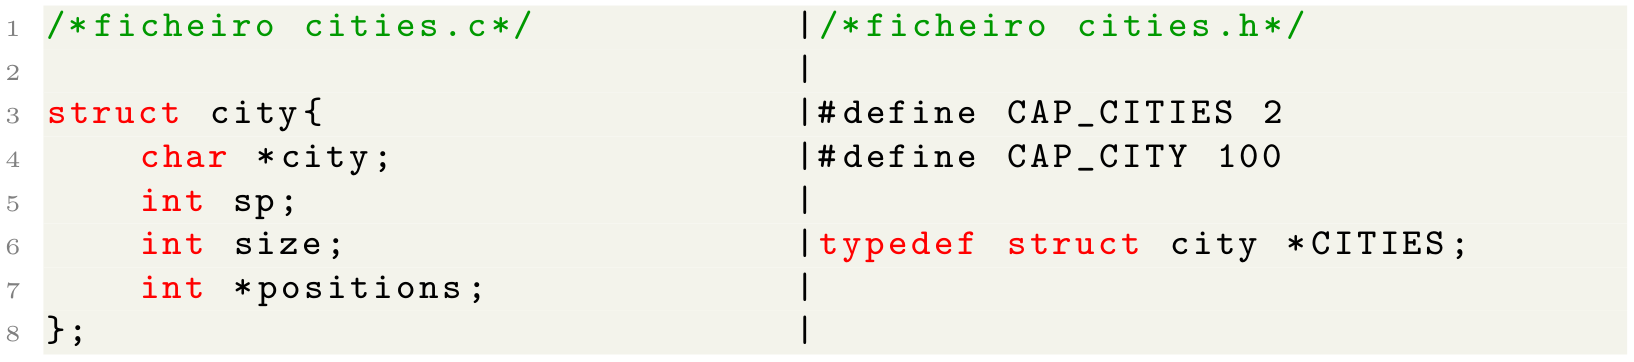
\includegraphics[width=1\linewidth]{images/cities.png}
        \caption*{Estrutura de dados das cidades}
        \label{fig:cities}
    \end{subfigure}
\end{figure}

Este módulo foi criado devido ao facto de o parâmetro "cidade" ser requerido em várias \textit{queries}, como tal, ao fazer uma busca de uma determinada cidade no \textit{array} \textbf{\small\texttt{RIDES}} seria necessário percorrer o \textit{array} todo, algo que levaria imenso tempo dado o elevadíssimo  tamanho do mesmo.

Portanto, para compensar tal debilidade, foi criada a seguinte estrutura, onde uma cidade possui um \textit{array} com todas as posições das suas ocorrências no \textit{array} \textbf{\small\texttt{RIDES}}, assim quando quisermos fazer uma busca, já sabemos previamente quais as posições que devemos analisar.



Ao verificar o código, vemos que o \textit{array} \textbf{\small\texttt{positions}} é um \textit{array} dinâmico de tamanho inicial definido por \textbf{\small\texttt{CAP\_CITY}}, e que possui um total de elementos definido pelo valor que o \textbf{\small\texttt{sp}} toma. Por fim, o \textit{array} \textbf{\small\texttt{CITIES}}  segue uma estrutura semelhante, onde \textbf{\small\texttt{CAP\_CITIES}} define o seu tamanho inicial e cada um dos seus elementos é uma \textbf{\small\texttt{struct city}}.

\section{Nota final}

Perante esta estrutura de dados certamente fica mais fácil responder às \textit{queries} em tempo útil, contudo uma das grandes desvantagens deve-se ao facto de esta estratégia ocupar demasiado espaço em memória, pois tanto os utilizadores, condutores e cidades armazenam todas as posições correspondentes às suas aparições no \textit{array} \textbf{\small\texttt{RIDES}}.


\chapter{Queries}

Durante a resolução das diversas consultas, procurámos sempre fazer tais operações no menor tempo possível, aproveitando ao máximo a estrutura de dados que tínhamos implementado, todavia a nossa implementação não se revelou a melhor para algumas das consultas, e portanto, enquanto algumas \textit{queries} podem ser facilmente resolvidas em tempo linear, outras são resolvidas em tempo quadrático, o que não é ótimo dado o elevado número de elementos que cada estrutura possui.

\section{Query 1}

A \textit{query} 1 consiste fundamentalmente em recolher a informação de um determinado utilizador ou condutor, isto conforme o primeiro parâmetro do \textit{input} seja uma \textit{string} de inteiros ou um \textit{username}. Assim sendo, a primeira fase da resolução deste problema passa por identificar qual o tipo de \textit{input} com que estamos a lidar, depois disso, podemos tirar partido do \textit{array} \textbf{\small\texttt{positions}} definido anteriormente, e a partir daí obtemos toda a informação necessária.    

\normalsize\textbf{Primeira fase }{\titlerule[0.5pt]}

Nesta fase temos de saber distinguir se um \textit{input} é referente a um utilizador ou condutor, como tal, decidimos aproveitar ao máximo a função \textbf{\small\texttt{atoi()}}, ou seja, como esta transforma uma \textit{string} num inteiro, se a \textit{string} apenas contiver inteiros vai ser devolvido o inteiro correspondente, por outro lado, se o primeiro carácter for uma letra do alfabeto a função vai retornar zero. Assim, desta forma, é possível distinguir um utilizador de um condutor.  

\normalsize\textbf{Segunda fase }{\titlerule[0.5pt]}

Como já sabemos qual a entidade em questão, resta-nos colocar o \textbf{\small\texttt{username}} do utilizador na função de \textit{hash} e obter o índice do \textit{bucket} para sabermos qual a lista que devemos percorrer. Assim, quando estivermos na célula correta, apenas teremos de guardar o \textit{array} \textbf{\small\texttt{positions}}, uma vez que este contem todas as posições do utilizador no \textit{array} \textbf{\small\texttt{RIDES}}.

Caso estejamos perante um condutor, muda o facto de podermos aceder ao mesmo em tempo constante, visto que este é mapeado conforme o seu \textbf{\small\texttt{id}}.

\normalsize\textbf{Terceira fase }{\titlerule[0.5pt]}

Depois de obtermos o \textit{array} \textbf{\small\texttt{positions}} já sabemos quais as posições que devemos analisar no \textit{array} \textbf{\small\texttt{RIDES}}, portanto, a partir daí basta recolher todos os dados necessários, quer para um utilizador, quer para um condutor.

\normalsize\textbf{Análise de complexidade }{\titlerule[0.5pt]}

Esta consulta tem uma complexidade pertencente a \(\theta(N)\), sendo que \(N\) corresponde ao número de viagens realizadas por um condutor ou utilizador.

\vspace{-6pt}
\section{Query 3}

Nesta busca, o objetivo consistia em listar um determinado número de utilizadores conforme a distância que estes tinham percorrido, como tal, é necessário calcular a distância total que cada um dos utilizadores percorreu para depois poder fazer uma análise comparativa.

\normalsize\textbf{Primeira fase }{\titlerule[0.5pt]}

Como os utilizadores estão numa tabela de \textit{hash} é necessário percorrer cada uma das listas ligadas para obter todos os dados, assim a primeira fase consiste em ir retornando os utilizadores conforme vamos percorrendo a tabela.

\normalsize\textbf{Segunda fase }{\titlerule[0.5pt]}

À medida que recebemos os utilizadores, podemos obter o \textit{array} \textbf{\small\texttt{positions}}. Daí segue que conseguimos fazer uma análise tendo apenas em conta os elementos do \textit{array} recebido, portanto basta aceder às posições indicadas e calcular o total acumulado das distâncias efetuadas nas viagens.

\normalsize\textbf{Terceira fase }{\titlerule[0.5pt]}

Assim que soubermos a distância percorrida por um utilizador, basta colocar esse mesmo utilizador e a sua distância num \textit{array}, a meio de fazermos uma ordenação e assim listar apenas o \textit{top} \(N\) utilizadores.

\normalsize\textbf{Análise de complexidade }{\titlerule[0.5pt]}

Esta consulta possui uma complexidade que pertencente a \(\theta(N^2)\), sendo que \(N\) simboliza o total de viagens que um utilizador fez. 


\section{Query 4}

Nesta consulta surge o desafio de calcular o preço médio das viagens numa dada cidade, algo que se torna bastante fácil dada a existência do módulo \textbf{\small\texttt{cities}}, uma vez que este contem os índices das viagens realizadas em cada uma das cidades.

\normalsize\textbf{Primeira fase }{\titlerule[0.5pt]}

Como nos é dada uma determinada cidade, basta procurar essa cidade no \textit{array} \textbf{\small\texttt{CITIES}} e retornar o \textit{array} \textbf{\small\texttt{positions}} correspondente, assim, desta forma, iremos aceder às posições exatas do \textit{array} \textbf{\small\texttt{RIDES}}.

\normalsize\textbf{Segunda fase }{\titlerule[0.5pt]}

Assim que obtivermos as posições que devemos analisar, basta aceder a essas posições e calcular o total acumulado do preço, para depois dividir pelo número de elementos do \textit{array} \textbf{\small\texttt{positions}}, assim descobrimos o preço médio das viagens numa determinada cidade.

\normalsize\textbf{Análise de complexidade }{\titlerule[0.5pt]}

Esta consulta possui uma complexidade pertencente a \(\theta(N)\), onde \(N\) representa o número de viagens realizadas numa dada cidade.

\section{Nota Final}

Durante a primeira fase do projeto o nosso grupo conseguiu realizar mais algumas \textit{queries}, contudo por questões de extensão do documento não nos é possível explicar as restantes consultas. Além disso, algumas delas, apesar de resolvidas, não estão do nosso agrado, e portanto também não faria sentido colocá-las aqui.

De qualquer modo, na segunda fase do projeto iremos focar a nossa análise nas \textit{queries} que não foram aqui mencionadas, a meio de fazermos um tratamento mais rigoroso do desempenho do programa. 




\chapter{Testes de Desempenho}


\begin{tabularx}{\textwidth} { 
  | >{\centering\arraybackslash}X 
  | >{\centering\arraybackslash}X 
  | >{\centering\arraybackslash}X | }
 \hline
 \textbf{\# Comando} & \textbf{Comando} & \textbf{Tempo de execução (s)} \\
 \hline
 \texttt{\textbf{1}} & \texttt{\textbf{1 PetrPacheco}} & \texttt{\textbf{0.000050}}  \\
 \hline
 \texttt{\textbf{2}} & \texttt{\textbf{1 ÂngVieira}} & \texttt{\textbf{0.000040}}  \\
 \hline
 \texttt{\textbf{3}} & \texttt{\textbf{1 LeTavares103}} & \texttt{\textbf{0.000021}}  \\
 \hline
 \texttt{\textbf{4}} & \texttt{\textbf{1 NoMaia}} & \texttt{\textbf{0.000021}}  \\
 \hline
 \texttt{\textbf{5}} & \texttt{\textbf{1 ErPinheiro7}} & \texttt{\textbf{0.000052}}  \\
 \hline
 \texttt{\textbf{6}} & \texttt{\textbf{1 FrederAraújo}} & \texttt{\textbf{0.000046}}  \\
 \hline
 \texttt{\textbf{7}} & \texttt{\textbf{1 PeFernandes144}} & \texttt{\textbf{0.000042}}  \\
 \hline
 \texttt{\textbf{8}} & \texttt{\textbf{1 ASousa7}} & \texttt{\textbf{0.000026}}  \\
 \hline
 \texttt{\textbf{9}} & \texttt{\textbf{1 RReis26}} & \texttt{\textbf{0.000022}}  \\
 \hline
 \texttt{\textbf{10}} & \texttt{\textbf{1 TerLima}} & \texttt{\textbf{0.000023}}  \\
 \hline
 \texttt{\textbf{11}} & \texttt{\textbf{1 000000002639}} & \texttt{\textbf{0.000012}}  \\
 \hline
 \texttt{\textbf{12}} & \texttt{\textbf{1 000000008561}} & \texttt{\textbf{0.000027}}  \\
 \hline
 \texttt{\textbf{13}} & \texttt{\textbf{1 000000004987}} & \texttt{\textbf{0.000026}}  \\
 \hline
 \texttt{\textbf{14}} & \texttt{\textbf{1 000000001936}} & \texttt{\textbf{0.000027}}  \\
 \hline
 \texttt{\textbf{15}} & \texttt{\textbf{1 000000003518}} & \texttt{\textbf{0.000043}}  \\
 \hline
 \texttt{\textbf{16}} & \texttt{\textbf{1 000000002581}} & \texttt{\textbf{0.000030}}  \\
 \hline
 \texttt{\textbf{17}} & \texttt{\textbf{1 000000004456}} & \texttt{\textbf{0.000027}}  \\
 \hline
 \texttt{\textbf{18}} & \texttt{\textbf{1 000000000879}} & \texttt{\textbf{0.000026}}  \\
 \hline
 \texttt{\textbf{19}} & \texttt{\textbf{1 000000009721}} & \texttt{\textbf{0.000032}}  \\
 \hline
 \texttt{\textbf{20}} & \texttt{\textbf{1 000000003558}} & \texttt{\textbf{0.000025}}  \\
 \hline
 \texttt{\textbf{21}} & \texttt{\textbf{3 50}} & \texttt{\textbf{0.253828}}  \\
 \hline
 \texttt{\textbf{22}} & \texttt{\textbf{4 Faro}} & \texttt{\textbf{0.018316}}  \\
 \hline
 \texttt{\textbf{23}} & \texttt{\textbf{4 Setúbal}} & \texttt{\textbf{0.013000}}  \\
 \hline
\end{tabularx}

\vspace{15pt}
\begin{center}
\begin{tabular}{ |p{4.73cm}|p{4.73cm}|p{4.73cm}|  }
 \hline
 \multicolumn{3}{|c|}{\textbf{Tempos para recolha de dados (s)}} \\
 \hline
 \centering\textbf{Utilizadores} & \hfil \textbf{Condutores} & \hfil \textbf{Viagens/Cidades} \\
 \hline
 \centering\textbf{\texttt{0.068262}} & \hfil \texttt{\textbf{0.022621}} & \hfil \texttt{\textbf{2.002561}}\\
 \hline
\end{tabular}
\end{center}

\end{document}
